\subsection{Módulo Encoder}
	\label{sec:encoder}
	
	El módulo \textit{Encoder} es el encargado de multiplexar los vectores de estado provenientes del módulo \textit{Network} y reconstruir una nueva trama, esta vez sin los valores de ocupación de vías por ser de sólo lectura. Esta nueva trama será \textit{packet}[N], junto con la señal \textit{processed} para indicar al módulo \textit{Printer} que la trama está completa y lista para ser transmitida. El diagrama de bloques de las máquinas de estado finitas con camino de datos se muestra en la Figura \ref{fig:Encoder_module}.
	
	\begin{figure}[H]
		\centering
		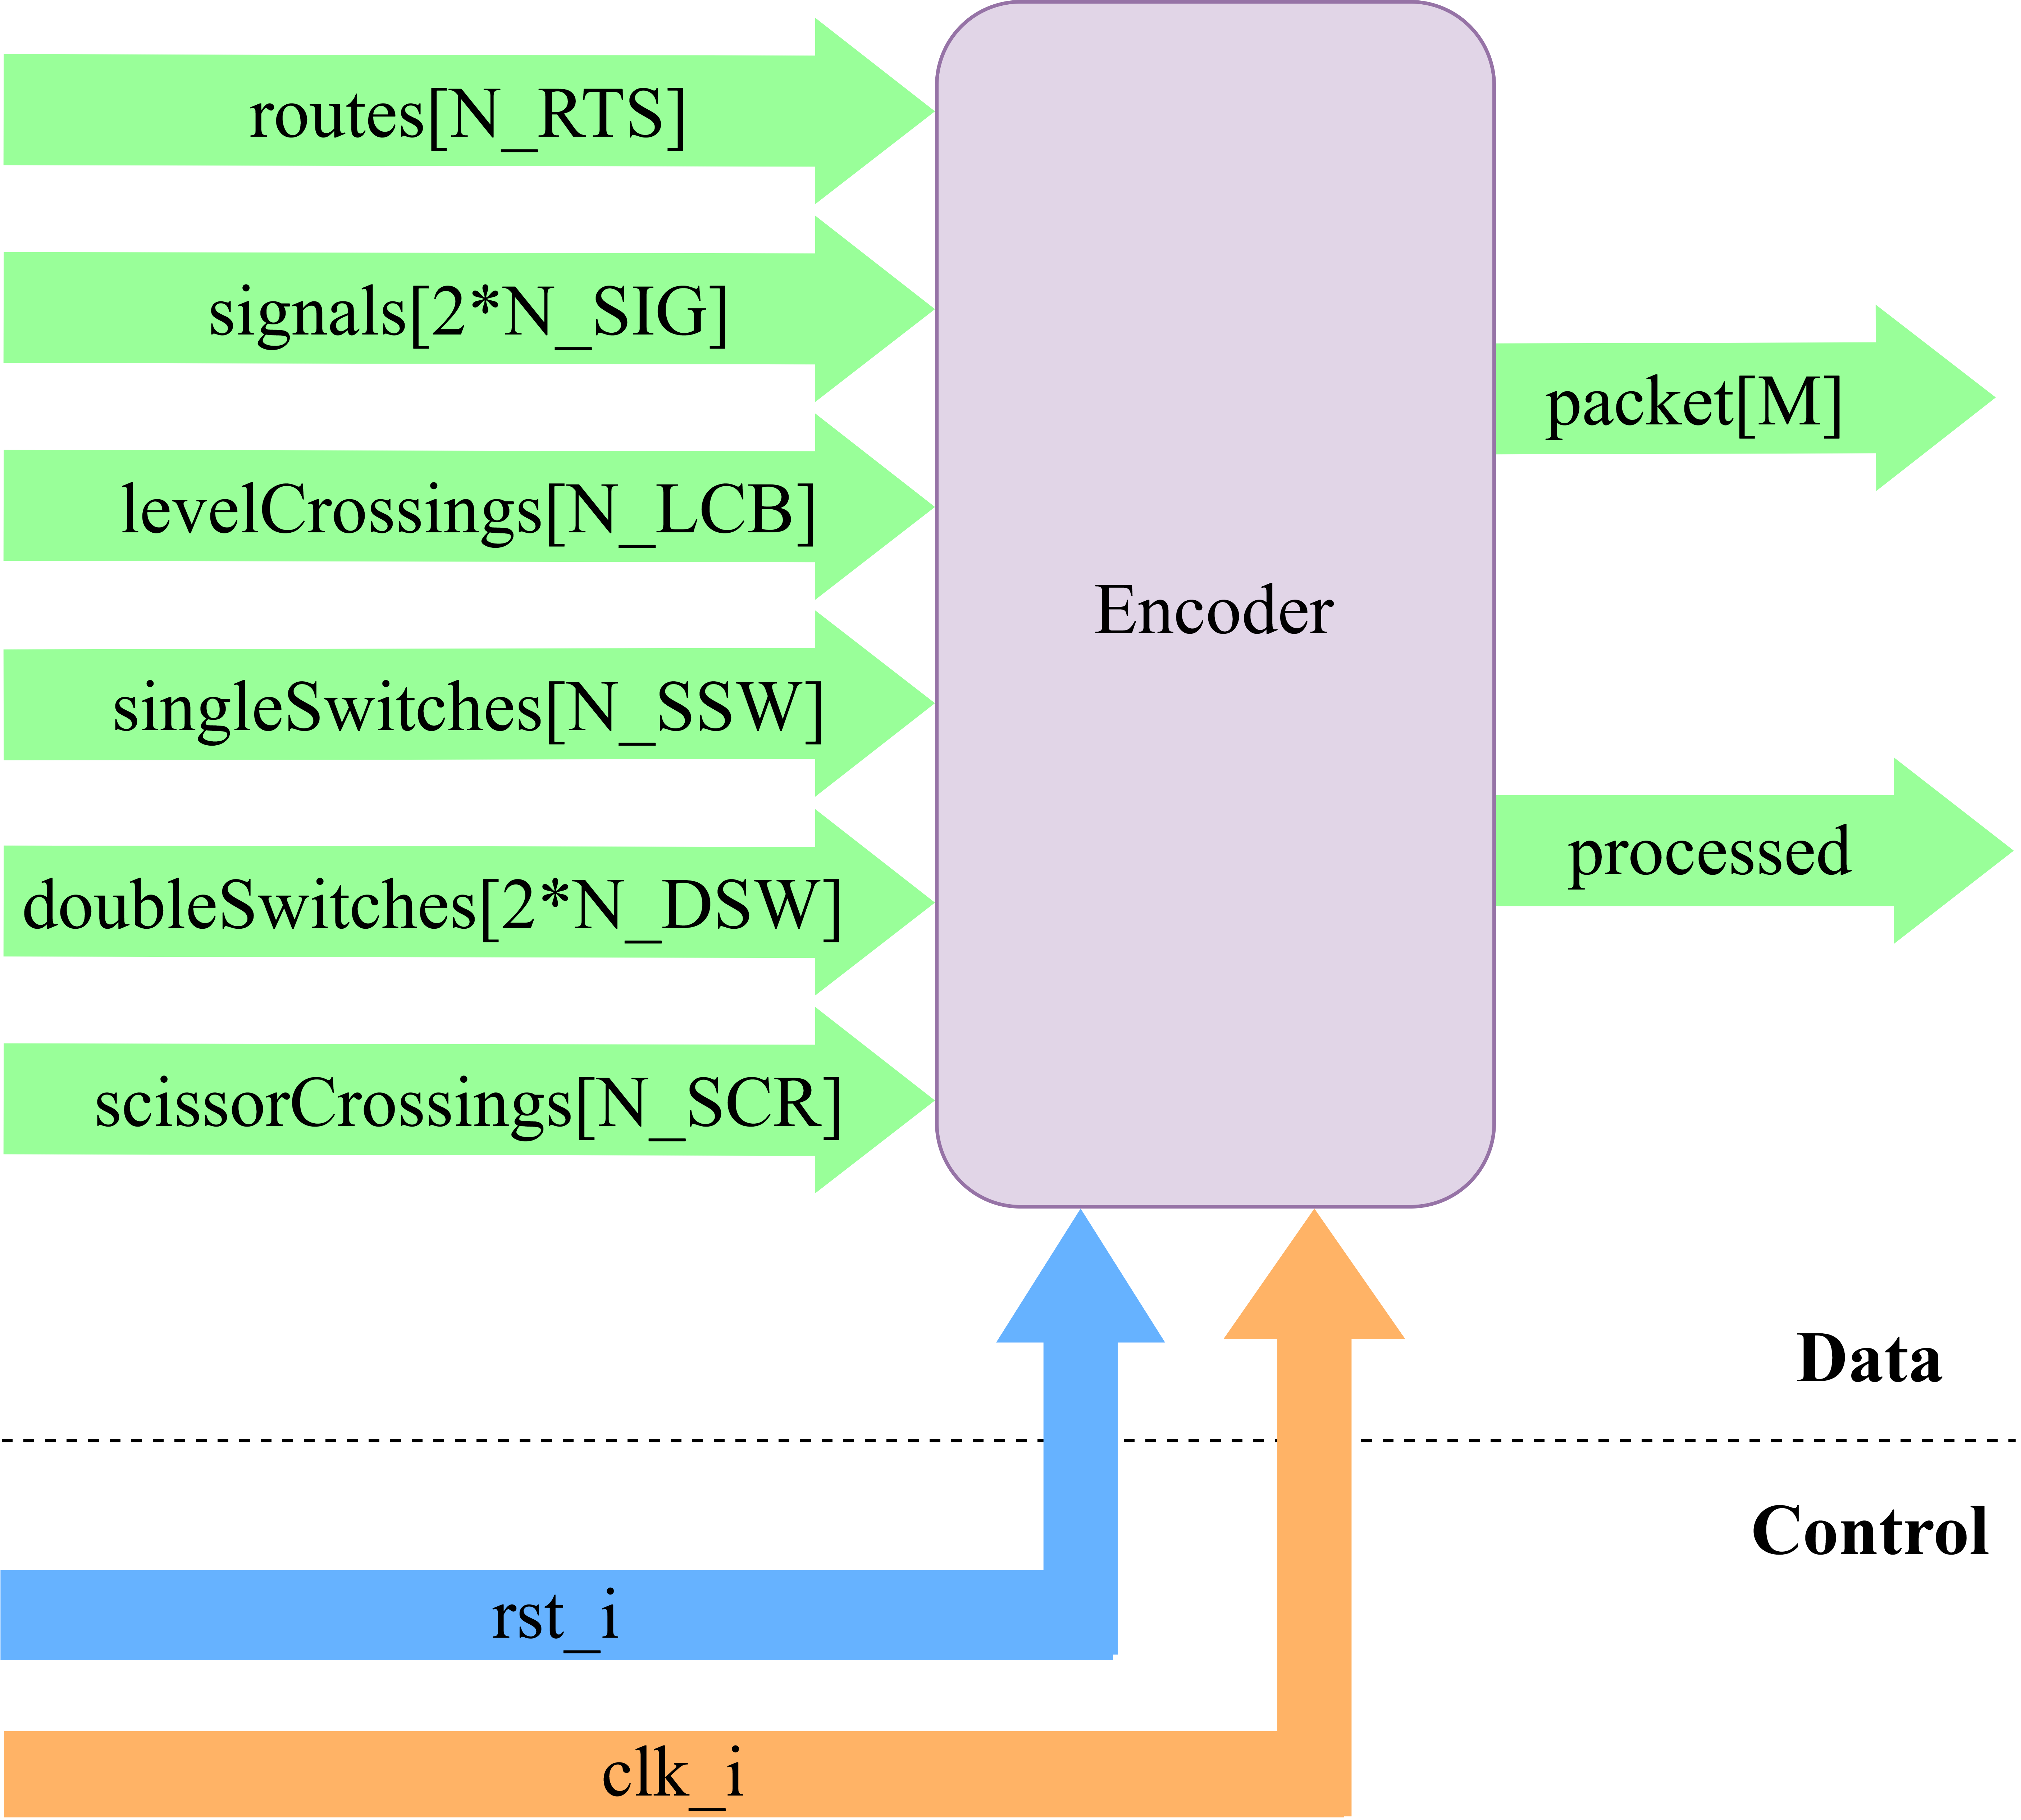
\includegraphics[width=1\textwidth]{Figuras/Encoder_module.png}
		\centering\caption{FSMD del módulo \textit{Encoder}.}
		\label{fig:Encoder_module}
	\end{figure}
	
	Al igual que la demultiplexación que realiza el módulo \textit{Decoder}, la multiplexación se basa en la cantidad de elementos ferroviarios de cada tipo, calculdos por el ACG al definir la trama tal cual fue explicado en la Sección \ref{sec:UART}. Los elementos inexistentes en la locación no serán tenidos en cuenta para formar la nueva trama, reduciendo el tamaño de la misma a su tamaño óptimo.